\section{Álgebra}

\questao{(Elaboração própria) Escreva a expressão algébrica que corresponde à sentença dada. Depois, determine o valor numérico dela para x = 12.}

O dobro de um número mais um terço desse mesmo número.

\begin{multicols}{4}
    \begin{enumerate}[label=\alph*) ]
        \item 24
        \item 28
        \item 27
        \item 34
    \end{enumerate}
\end{multicols}

% Caso a questão tenha mais de uma solução, alterar o valor da segunda chaves, que se refere ao valor para a quantidade de soluções que a questão terá.
% e insira o comando \solucao para uma nova resolução do item.
\begin{solucoes}{1}
\solucao

    Primeiro, transformamos a linguagem usual em linguagem matemática, assim, temos a seguinte expressão algébrica:

    \begin{equation*}
        2x + \cfrac{1}{3}\times x
    \end{equation*}

    Substituindo o valor dado na questão, temos:
    
    \begin{equation*}
        2 \times 12 + \cfrac{1}{3} \times 12 = 24 + \cfrac{12}{3} = 24 + 4 = 28
    \end{equation*}

    Então, o valor numérico da expressão algébrica é 28. \\
    \textbf{ALTERNATIVA B)}
\end{solucoes}

\questao{(OM$^3$SP 2026 - 1ª Fase) Em um dia na E.M.M.M.S.P. a diretora Sheyla propôs um desafio matemático. Aquele que acertasse seria dispensado de suas duas últimas aulas. Ela propôs o seguinte desafio: \textquotedblleft Vinte rapaduras custam $R\$ \ 60,00$ a mais do que cinco rapaduras. Qual o valor de uma rapadura?\textquotedblright\, Pensando na dispensa das duas últimas aulas, qual é o valor de uma rapadura?}
        \begin{multicols}{4}
            \begin{enumerate}[label=\alph*)]
                \item $R\$ \ 3,50$
                \item $R\$ \ 4,00$
                \item $R\$ \ 4,50$
                \item $R\$ \ 5,00$
            \end{enumerate}
        \end{multicols}

\begin{solucoes}{2}
    \solucao
    Temos aqui um problema clássico da álgebra e para resolvermos utilizaremos como método de solução uma equação do  primeiro grau. A diretora Sheyla propôs que vinte rapaduras custam $R\$ \ 60,00$ a
mais do que cinco rapaduras. Não sabemos o valor de cada rapadura, assim chame o número de rapaduras de $x$ e assim teremos:
\begin{equation*}
20x=60+5x
\end{equation*}
\begin{equation*}
20x-5x=60
\end{equation*}\begin{equation*}
15x=60
\end{equation*}
\begin{equation*}
x=\frac{60}{15}
\end{equation*}
\begin{equation*}
x=4.
\end{equation*}
Logo, o valor de cada rapadura é $R\$ \ 4,00$.\\
\textbf{ALTERNATIVA B)}

\solucao
Muitas vezes existe uma dificuldade de observação frente aos problemas algébricos. Mas, é possível resolvê-lo sem necessariamente saber montar uma equação. O enunciado nos diz que vinte rapaduras custam o mesmo que cinco rapaduras mais $R\$ \ 60,00$. Com isso, podemos perceber que se subtrairmos as vinte rapaduras das outras cinco, teremos a quantidade de rapaduras que valem exatamente $R\$ \ 60,00$. Logo, $20-5=15$ e assim descobrimos que $15$ rapaduras equivalem a $R\$ \ 60,00$. Para descobrir o valor de uma rapadura, é só dividir os $R\$ \ 60,00$ por $15$. Como, $\frac{60}{15}=4$, então uma rapadura vale exatamente $R \$ \ 4,00$ \\
    \textbf{ALTERNATIVA B)}
\end{solucoes}

\questao{(OM$^3$SP 2026 - 1ª Fase)Os números triangulares foram sistematizados pela escola pitagórica. Esses números são representados, com exceção do primeiro, por triângulos equiláteros (triângulos com os três lados iguais). Na imagem abaixo estão os cinco primeiros números triangulares:}
        \begin{figure}[H]
            \centering
            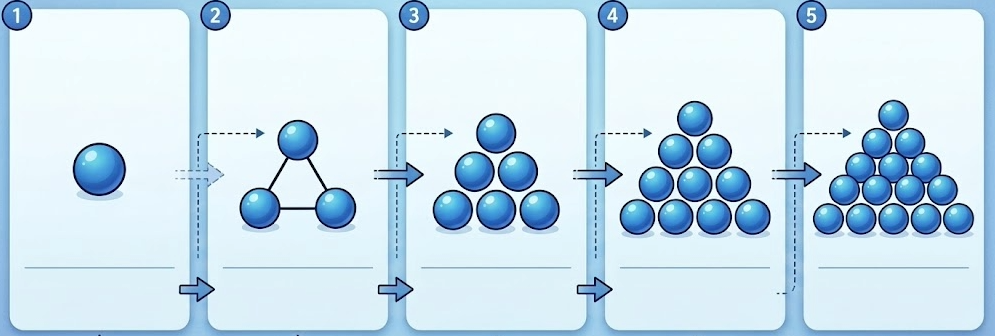
\includegraphics[width=0.9\linewidth]{figuras/7_ano/Números Triangulares.png}
        \end{figure}
        Qual o número de bolinhas no oitavo número triangular?
        \begin{multicols}{4}
            \begin{enumerate}[label=\alph*)]
                \item $21$
                \item $28$
                \item $36$
                \item $45$
            \end{enumerate}
        \end{multicols}

\begin{solucoes}{2}
    \solucao 
Os números triangulares são números interessantíssimos. Percebemos que os números triangulares estão dispostos em uma sequência numérica da seguinte forma: $T_n=\{1,3,6,10,15,...\}$. Agora, é preciso que encontremos o oitavo número triangular. Se percebermos o padrão de crescimento, veremos que do $1^\circ$ para o $2^\circ$ aumentou-se em duas unidades. Do $2^\circ$ para o $3^\circ$ aumentou-se em três unidades e assim por diante. Logo,
        \begin{equation*}
        T_6=15+6=21
        \end{equation*}
         \begin{equation*}
        T_7=21+7=28
        \end{equation*}
         \begin{equation*}
        T_8=28+8=36
        \end{equation*}
        o $8^\circ$ número triangular é o 36. \\
    \textbf{ALTERNATIVA C)}

    \solucao
    Os números triangulares são números interessantíssimos. Percebemos que os números triangulares estão dispostos em uma sequência numérica da seguinte forma: $T_n=\{1,3,6,10,15,...\}$. Agora, é preciso que encontremos o oitavo número triangular. Se percebermos o padrão de crescimento, veremos que $T_2=1+2$, $T_3=1+2+3$, $T_4=1+2+3+4$ e $T_5=1+2+3+4+5$. Sendo assim, podemos modular o termo geral da seguinte forma:
        
        \begin{equation*}
        T_n=1+2+3+4+...+(n-1)+n \\\\\\\ (1)
        \end{equation*}
        \begin{equation*}
        T_n=n+(n-1)+...+4+3+2+1 \\\\ (2)
 \end{equation*}
        
        somando $(1)$ e $(2)$:
        \begin{equation*}
        2T_n=(n+1)+(n+1)+...+(n+1)
        \end{equation*}
        \begin{equation*}
        2T_n=n\cdot(n+1)
        \end{equation*}
        \begin{equation*}
        T_n=\frac{n\cdot(n+1)}{2})
        \end{equation*}
        Logo, para determinar o oitavo número triangular substituiremos $n=8$. Com isso, 
        \begin{equation*}
            T_8=\frac{8\cdot(8+1)}{2}=\frac{8\cdot 9}{2}=\frac{72}{2}=36
        \end{equation*}
        Portanto, o $8^\circ$ número triangular é o 36. \\
    \textbf{ALTERNATIVA C)}
\end{solucoes}

\questao{(OM$^3$SP 2026 - 1ª Fase) O ring do UFC tem o formato de um octágono. O professor Samuel fez a medida dos lados do ring, mas para trabalhar os princípios algébricos, trocou o valor numérico por letras. Qual será o perímetro do ring considerando os lados apresentados na figura abaixo?}
        \begin{figure}[H]
            \centering
            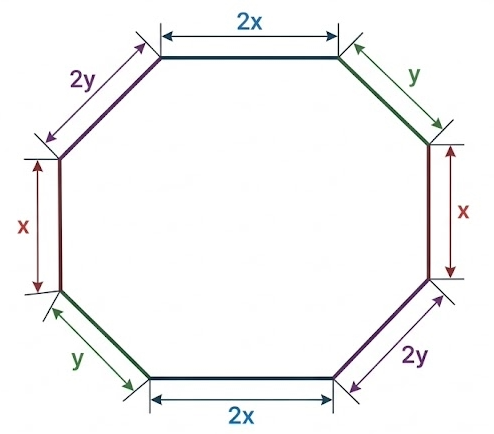
\includegraphics[width=0.5\linewidth]{figuras/7_ano/Perímetro.png}
        \end{figure}
        \begin{multicols}{4}
            \begin{enumerate}[label=\alph*)]
                \item $6x+6y$
                \item $6x+4y$
                \item $4x+6y$
                \item $4x+4y$
            \end{enumerate}
        \end{multicols}

\begin{solucoes}{1}
    \solucao
    
    Para resolver esta questão é preciso recordar a noção de perímetro. O prerímetro é a soma de todos os lados da figura e assim teremos:
        \begin{equation*}
            2P=2x+y+x+2y+2x+y+x+2y
        \end{equation*}
        e ao reduzir os termos iguais,
        \begin{equation*}
            2P=6x+6y.
        \end{equation*}
        Então, o perímetro deste ring vale 
        $6x+6y$.  \\
    \textbf{ALTERNATIVA A)}
\end{solucoes}

\questao{(OM$^3$SP 2026 - 1ª Fase)Ao ler o jornal pela manhã o coordenador Jefferson observou uma notícia intrigante:\\\\
        \textbf{No último sábado foi calculado uma preciptação de 150mm a mais do que a preciptação da sexta-feira. Além disso, no domingo foi calculado uma preciptação de 30mm a menos que na sexta-feira}. \\\\ O coordenador Jefferson lembrou que no sábado choveu 200mm. Sendo assim, quanto choveu no domingo?}
        \begin{multicols}{4}
            \begin{enumerate}[label=\alph*)]
                \item $50mm$
                \item $40mm$
                \item $30mm$
                \item $20mm$
            \end{enumerate}
        \end{multicols}
\begin{solucoes}{2}
\solucao
    Olhando para a manchete que o coordenador Jefferson leu, podemos ver que, (considere sexta como $x$, sábado como $y$ e domingo como $z$)
        \begin{equation*}
            y=x+150 \ (1)
        \end{equation*}
        \begin{equation*}
              z=x-30. \ (2)
        \end{equation*}
        Jefferson sabia que a precipitação de sábado foi de $200mm$, ou seja, $y=200$. Substituindo esta informação em $(1)$,
        \begin{equation*}
            200=x+150 \Longrightarrow x=50mm. \ (3)
        \end{equation*}
        Assim, por $(3)$, a precipitação de sexta foi de $50mm$. Por fim, substituindo $
        (3)$ em $(2)$,
        \begin{equation*}
            z=50-30=20mm. \ (4)
        \end{equation*}
Assim, por $(4)$, no domingo a precipitação foi de $20mm$. \\
    \textbf{ALTERNATIVA D)}

\solucao

Muitos discentes possuem dificuldades coma linguagem algébrica e podemos resolver este problema sem necessariamente precisarmos montar as expressões algébricas. Sabemos que no sábado choveu $200mm$ e que no sábado choveu $150mm$ a mais que na sexta, então na sexta choveu $200m-150mm=50mm$. Sabemos também que no domingo choveu $30mm$ a menos que na sexta, assim $50mm30mm=20mm$. Logo,no domingo, a preciptação foi de $20mm$.   \\
    \textbf{ALTERNATIVA D)}

\end{solucoes}

\questao{(OM$^3$SP 2026 - 1ª Fase)O professor Jadiel gosta muito de comer salgadinho de padaria. Todavia, por comer muito, teve uma orientação nutricional de diminuir a quantidade de salgadinho ingerido até não comer mais nenhum. No primeiro dia ele comeu 45 salgadinhos, no segundo dia ele comeu 44 salgadinhos, no terceiro dia ele comeu 42 salgadinhos, no quarto dia ele comeu 39 salgadinhos e assim por diante. Em qual dia ele deixou de comer os salgadinhos?}
         \begin{multicols}{4}
            \begin{enumerate}[label=\alph*)]
                \item $6^\circ$  dia
                \item $8^\circ$ dia
                \item $10^\circ$  dia
                \item $12^\circ$  dia
            \end{enumerate}
        \end{multicols}

\begin{solucoes}{2}
\solucao
A questão nos deu os seguintes números: $S_n=\{45,44,42,39,...\}$. Agora, é preciso que encontremos o dia em que o professor Jadiel parou de comer salgadinhos. Se percebermos o padrão de decrescimento, veremos que do $1^\circ$ para o $2^\circ$ diminuiu-se em uma unidade. Do $2^\circ$ para o $3^\circ$ diminuiu-se em duas unidades e assim por diante. Logo,
 \begin{equation*}
     S_5=39-4=35
 \end{equation*}
  \begin{equation*}
     S_6=35-5=30
 \end{equation*}
 \begin{equation*}
     S_7=30-6=24
 \end{equation*}
  \begin{equation*}
     S_8=24-7=17
 \end{equation*}
 \begin{equation*}
     S_9=17-8=9
 \end{equation*}
  \begin{equation*}
     S_{10}=9-9=0
 \end{equation*}
 Logo, no décimo dia o professor Jadiel parará de comer salgadinhos.   \\
    \textbf{ALTERNATIVA C)}

\solucao
Podemos pensar também algebricamente. Tem-se aí um princípio de sequência de termos onde o próximo termo é sempre o anterior subtraido de um mesmo número, no caso o número $1$. Queremos determinar o tempo $n$ para $a_n=o$. Agora, é preciso que encontremos o oitavo número triangular. Se percebermos o padrão de crescimento, veremos que $a_2=45-1$, $a_3=45-1-2$, $a_4=45-1-2-3$ e $a_5=45-1-2-3-4$. Sendo assim, podemos modular o termo geral da seguinte forma:
  
        \begin{equation*}
        a_n=45-1-2-3-...-(n-1) \ 
        \end{equation*}
        \begin{equation*}
        a_n=45-(1+2+3+4+5+...+n-1)
 \end{equation*}
 \begin{equation*}
     a_n= 45-\frac{(n-1)*n}{2}
 \end{equation*}
        
Logo, como queremos mostrar o valor de $n$ para que $a_n$ seja $0$, faremos
\begin{equation*}
    0=45-\frac{(n-1)*n}{2}
\end{equation*}
\begin{equation*}
    \frac{(n-1)*n}{2}=45
\end{equation*}
\begin{equation*}
    (n-1)*n=90
\end{equation*}
\begin{equation*}
    (n-1)*n=9*10
\end{equation*}
\begin{equation*}
    (n-1)*n=(10-1)*10
\end{equation*}

Sendo assim, $n=10$. Logo, no décimo dia o professor Jadiel parará de comer salgadinhos. 
\\
\textbf{ALTERNATIVA C)}
\end{solucoes}

\questao{(OAM 2025 - NÍVEL 1) Os múltiplos de 3 foram escritos seguindo o padrão da figura ao lado. Sabe-se que Clarisse continuou escrevendo até a décima linha e depois somou o primeiro com o último número que aparecem nessa linha. Qual o valor encontrado por Clarisse?}
\begin{figure}[H]
    \centering
    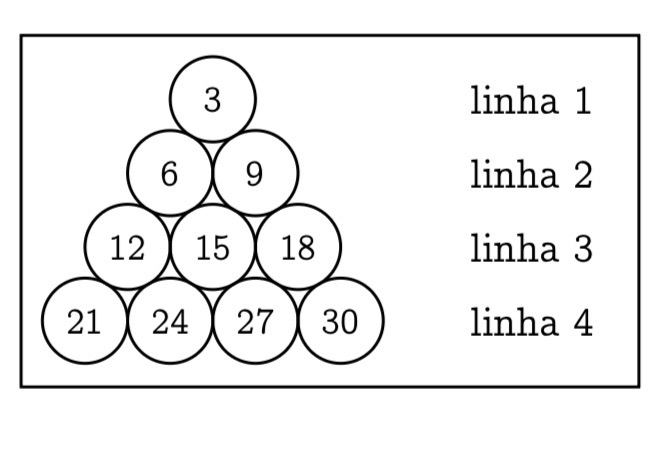
\includegraphics[width=0.5\linewidth]{figuras/7_ano/IMG_0943.jpeg}
    \label{fig:placeholder}
\end{figure}

\begin{solucoes}{2}
    \solucao
    Vemos na imagem abaixo um padrão claro, os números são formados pelos múltiplos de três em sua ordem. A imagem é bem clara na sequência de termos e percebemos que cada bola está na sequência de múltiplos de $3$. Cada linha tem exatamente o mesmo número de bolas do número da linha. A linha quatro possui $3\cdot 7=21$, $3\cdot8=24$, $3\cdot 9=27$ e $3\cdot 10=30$. Podemos determinar a sequência a partir da quinta linha e irmos até a décima:
\\\\
    $i)$ Linha 5
\\\\
    $3\cdot 11=33$, $3\cdot 12=36$, $3\cdot 13=39$, $3\cdot 14=42$, $3\cdot 15=45$.
\\\\
    $ii)$ Linha 6
\\\\
    $3\cdot 16=48$, $3\cdot 17=51$, $3\cdot 18=54$, $3\cdot 19=57$, $3\cdot 20=60$ e $3\cdot 21=63$.
\\\\
    $iii)$ Linha 7
\\\\
    $3\cdot 22=66$, $3\cdot 23=69$, $3\cdot 24=72$, $3\cdot 25=75$, $3\cdot 26=78$, $3\cdot 27=81$ e $3\cdot 28=84$.
\\\\
    $iv)$ Linha 8
\\\\
    $3\cdot 29=87$, $3\cdot 30=90$, $3\cdot 31=93$, $3\cdot 32=96$, $3\cdot 33=99$, $3\cdot 34=102$, $3\cdot 35=105$ e $3\cdot36=108$.
\\\\
    $v)$ Linha 9
\\\
       $3\cdot 37=111$, $3\cdot 38=114$, $3\cdot 39=117$, $3\cdot 40=120$, $3\cdot 41=123$, $3\cdot 42=126$, $3\cdot 43=129$, $3\cdot 44=132$ e $3\cdot45=135$.
\\\\
    $vi)$ Linha 10
\\\\
    $3\cdot 46=138$, $3\cdot 47=141$, $3\cdot 48=144$, $3\cdot 49=147$, $3\cdot 50=150$, $3\cdot 51=153$, $3\cdot 52=156$, $3\cdot 53=159$, $3\cdot 54=162$ e $3\cdot 55=165$.
\\\\
Queremos a soma do primeiro e do último da linha 10, assim $138+165=303$.

\solucao
Se pensarmos aqui temos uma sequência de termos que possui uma razão constante (enrolando um pouco para não utilizar o termo progressão aritmética). Logo, se pensarmos em termo geral, temos que todos os elementos são múltiplos de 3. Logo $a_n=3\cdot n$. Para descobrir o último termo podemos pensar da seguinte maneira apenas somando as linhas $1+2+3+4+5+6+7+8+9+10=55$ e teríamos que o último termo é $a_{55}=3\cdot 55=165$ e o primeiro termo da linha seria o $a_{46}=3\cdot 46=138$. Assim, $138+165=303$.

\end{solucoes}
